\section{Top Quark and Higgs Decay}
\label{problem_and_app}

In the LHC, two proton beams are accelerated close to the speed of light in opposite directions, set to collide inside a specific particle detector. From this head-on collision results a chain reaction of decaying particles, and most of the final particles react with the detector allowing their characteristics to be recorded. One of the experiments being conducted at the ATLAS detector is related to the studies of top quark and Higgs boson properties. Figure \ref{fig:ttbar} presents the schematic representation of the top quark decay (addressed as the \ttbar system).

\begin{figure}[!htp]
	\begin{center}
		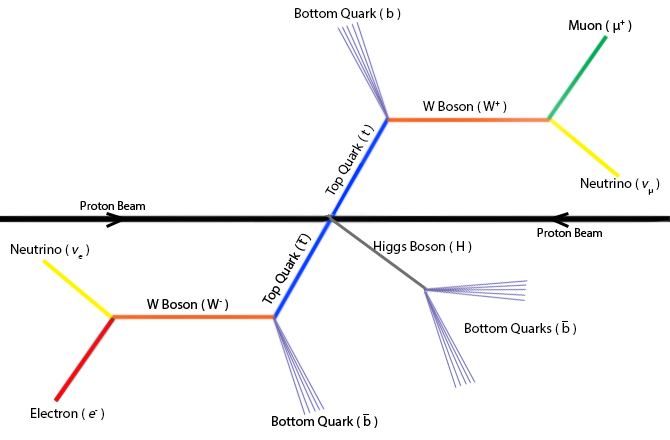
\includegraphics[scale=0.4]{images/ttbar_higgs.png}
		\caption{Schematic representation of the \ttbar system and Higgs boson decay.}
		\label{fig:ttbar}
	\end{center}
\end{figure}

The ATLAS detector can record the characteristics of the bottom quarks, detected as a jet of particles, and leptons (muon and electron). However, neutrinos do not interact with the detector and, therefore, their characteristics are not recorded. Since the top quark reconstruction requires the neutrinos, their characteristics are analytically determined with the known information of the system, in a process known as kinematical reconstruction. However, the \ttbar system may not have a possible reconstruction. The reconstruction has a degree of certainty associated, which determines its quality.

The amount of Bottom quark jets and leptons detected may vary between events, due to other reactions occurring alongside the top quark decay. As represented in figure \ref{fig:ttbar}, 2 jets and 2 leptons are needed to reconstruct the \ttbar system, but the input data for an event may have many more of these particles associated. It is necessary to reconstruct the system for every combination of 2 jets and 2 leptons in the input data (referred only as combination). Then, only the most accurate reconstruction of each event is considered.

The Higgs boson is reconstructed from the two jets that it decays to, but only if the \ttbar system as a possible reconstruction. This adds at least two more jets to the event information, increasing the number of possible combinations, as they are the same as the \ttbar system jets. The Higgs boson reconstruction uses the jets that were not needed in the \ttbar system. The overall quality of the event reconstruction depends on the quality of both \ttbar system and Higgs boson reconstructions.

The ATLAS detector has an experimental resolution that induces an error of 2\% in each measure of the particle characteristics. This error is propagated into the \ttbar system and Higgs reconstructions, affecting their accuracy. To improve the quality of the reconstructions a random variation to the particles parameters is applied, with a maximum magnitude of 2\%, a given amount of times and chose the event reconstruction with the highest accuracy. The quality of the reconstructions and application execution time are directly proportional to the amount of variations performed per combination. The goal is to do as many variations as possibly within a reasonable time frame.

The \tth application was designed to reconstruct of the \ttbar system and Higgs boson, as explained above. The application flow is presented in figure \ref{fig:flow}. Each event on the input file is individually loaded to a single global state shared among the application and the LipMiniAnalysis library, and it is overwritten every time a new event is loaded. The event is then submitted to a series of cuts, which filters events that are not suited for reconstruction. When an event reaches the cut 20 the \ttbar system and Higgs boson are reconstructed in a function named \ttDilepKinFit. If the \ttbar system reconstruction fails, the current combination is discarded and the next is processed. If an event has a possible reconstruction it passes the final cut and its final information is stored.

\begin{figure}[!htp]
	\begin{center}
		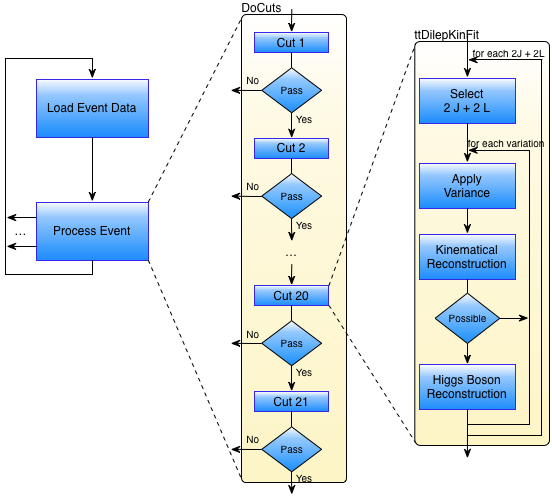
\includegraphics[scale=0.4]{images/graf_abstract_flow_with_kinfit.png}
		\caption{Schematic representation for the \tth application flow.}
		\label{fig:flow}
	\end{center}
\end{figure}
